\documentclass[11pt,a4paper]{amsart}

%% ─── Encoding & language ───────────────────────────────────────────
\usepackage[T1]{fontenc}
\usepackage[utf8]{inputenc}
\usepackage[english]{babel}

%% ─── Typography ────────────────────────────────────────────────────
\usepackage{microtype}
\usepackage{csquotes}

%% ─── Mathematics ───────────────────────────────────────────────────
\usepackage{amsmath, amssymb, amsthm}
\numberwithin{equation}{section}

%% ─── Page layout ───────────────────────────────────────────────────
\raggedbottom

%% ─── Lists, tables, figures & algorithms ──────────────────────────
\usepackage{enumitem}
\usepackage{booktabs}
\usepackage{graphicx}
\graphicspath{{project/figures/}}
\usepackage{algorithm}
\usepackage[noend]{algpseudocode}

%% ─── Bibliography ──────────────────────────────────────────────────
\usepackage[
  backend=biber,
  style=numeric-comp,
  sorting=none,
  giveninits=true,
  doi=true,
  url=false,
  isbn=false,
  eprint=true,
  maxbibnames=99,
  maxcitenames=2
]{biblatex}
\addbibresource{seminar.bib}
\AtEveryBibitem{\clearlist{language}}
\renewcommand*{\bibfont}{\normalfont\footnotesize}  % amsart's \bibliofont
\renewcommand*{\postnotedelim}{\addcomma\addnbspace}
\AtBeginBibliography{\setlength{\emergencystretch}{1em}}

%% ─── Hyperlinks & metadata ─────────────────────────────────────────
\usepackage{hyperref}
\hypersetup{
  colorlinks=true,
  linkcolor=black,
  citecolor=blue,
  urlcolor=blue,
  pdftitle={The EM Algorithm for Gaussian Mixtures},
  pdfauthor={Elvir Muslić}
}
\usepackage{orcidlink}

%% ─── Theorem environments ─────────────────────────────────────────
\theoremstyle{plain}
\newtheorem{theorem}{Theorem}[section]
\newtheorem{proposition}[theorem]{Proposition}
\newtheorem{lemma}[theorem]{Lemma}
\newtheorem{corollary}[theorem]{Corollary}

\theoremstyle{definition}
\newtheorem{definition}[theorem]{Definition}
\newtheorem{example}[theorem]{Example}

\theoremstyle{remark}
\newtheorem{remark}[theorem]{Remark}

%% ─── Algorithms ───────────────────────────────────────────────────
\algrenewcommand\algorithmicrequire{\textbf{Input:}}
\algnewcommand{\IfThen}[2]{\State \algorithmicif\ #1\ \algorithmicthen\ #2}

%% ─── Notation shortcuts ───────────────────────────────────────────
\newcommand{\R}{\mathbb{R}}
\newcommand{\N}{\mathcal{N}}
\newcommand{\T}{\mathsf{T}}
\newcommand{\given}{\mid}
\newcommand{\code}[1]{\texttt{#1}}

\begin{document}

%% ─── Seminar cover page ───────────────────────────────────────────
\thispagestyle{empty}
\begin{center}
  {\large University of Niš\par}
  {\large Faculty of Sciences and Mathematics\par}
  \smallskip
  Department of Computer Science\par
  Doctoral Academic Studies in Computer Science\par

  \vspace{3em}
  {\itshape Seminar paper\par}
  {\itshape Course: Machine Learning (20.IDI12)\par}

  \vspace{3.5em}
  \rule{\linewidth}{0.4pt}\par
  \vspace{1em}
  {\LARGE\bfseries The EM Algorithm\\[0.35em]
    for Gaussian Mixtures\par}
  \vspace{1em}
  \rule{\linewidth}{0.4pt}\par
\end{center}

\vspace{3.5em}
\noindent
\begin{minipage}[t]{0.49\linewidth}
  \raggedright
  \textbf{Mentor}\par
  Prof.\ Branimir Todorović
\end{minipage}\hfill
\begin{minipage}[t]{0.49\linewidth}
  \raggedleft
  \textbf{Student}\par
  Elvir Muslić\,\orcidlink{0009-0006-4042-6550}\par
  ORCID \href{https://orcid.org/0009-0006-4042-6550}{0009-0006-4042-6550}
\end{minipage}

\vfill
\begin{center}Niš, October 2026\end{center}
\newpage

%% ─── Abstract & front information ─────────────────────────────────
\begin{center}\scshape Abstract\end{center}
\noindent
A Gaussian mixture models data that fall into groups without labels:
each group is a Gaussian, and the group of each point is hidden. Its
log-likelihood has no closed-form maximizer, and the
expectation-maximization (EM) algorithm climbs it in two closed-form
steps. The E-step computes, by Bayes' rule, the responsibility of each
component for each point, and the M-step refits each component with
these responsibilities as weights. This paper presents the model and the
algorithm, works through one iteration by hand, and explains why no
iteration lowers the log-likelihood. The estimator
\code{GaussianMixture} of scikit-learn reproduces the hand iteration to
$6.2 \cdot 10^{-15}$. On the Old Faithful data, EM from a poor start
first makes the two components almost identical, leaves this state
slowly, and converges after $53$ iterations; twenty random starts all
reach the same log-likelihood of the standardized data, $-385.4607$.

\bigskip
\setcounter{tocdepth}{1}
\tableofcontents

%% ═══════════════════════════════════════════════════════════════════
\section{Introduction}\label{sec:intro}

The Old Faithful geyser in Yellowstone National Park erupts at irregular
intervals. The data set \code{faithful} of R records $272$ eruptions,
each by its duration and by the waiting time to the next eruption, in
minutes; Azzalini and Bowman~\cite{azzalini1990} analyze a more complete
version of this record. Plotted, the eruptions fall into two groups,
short eruptions followed by short waits and long ones followed by long
waits (Figure~\ref{fig:iterations}(d)). No eruption is labeled with its
group, and finding the groups from the points alone is the task of
clustering.

A model makes the task precise. A Gaussian mixture describes each group
by a Gaussian distribution, with its own center, spread and share of the
data, and gives every point a probability of belonging to each group
instead of a hard label. Its parameters are fitted by maximum
likelihood, which has no closed-form solution here, no formula that
gives the parameters directly, because the labels are missing. The
expectation-maximization (EM) algorithm of Dempster,
Laird and Rubin~\cite{dempster1977} fills the labels in with
probabilities, refits the groups, and repeats~\cite{bishop2006,
mclachlan2008}. The paper does four things.
\begin{enumerate}[leftmargin=*, nosep]
\item Section~\ref{sec:model} presents the Gaussian mixture and its
  log-likelihood.
\item Section~\ref{sec:em} presents the two steps of EM and its
  algorithm, and carries out one iteration by hand.
\item Section~\ref{sec:theory} explains why no iteration lowers the
  log-likelihood, and where EM can stop.
\item Section~\ref{sec:experiments} runs EM with
  scikit-learn~\cite{pedregosa2011} on Old Faithful, checked against the
  hand iteration.
\end{enumerate}

%% ═══════════════════════════════════════════════════════════════════
\section{The Gaussian Mixture}\label{sec:model}

\subsection{The Gaussian}\label{sec:gaussian}

A Gaussian, or normal, distribution in $\R^d$ has two parameters. Its
\emph{mean} $\mu \in \R^d$ is the center of its points. Its
\emph{covariance} $\Sigma$, a symmetric $d \times d$ matrix, with a
positive variance in every direction, describes their spread: the
diagonal holds the variance of each coordinate, and an off-diagonal
entry says how two coordinates vary together, positive when they tend to
grow together.

The density $\N(x \given \mu, \Sigma)$ is proportional to
$\exp\bigl(-\tfrac12 (x - \mu)^\T \Sigma^{-1} (x - \mu)\bigr)$: it is
largest at $\mu$ and falls off with the distance from $\mu$, measured in
units of the spread in each direction. Points of equal density lie on
ellipses centered at $\mu$ (ellipsoids if $d > 2$), stretched along the
directions in which the points spread most;
Figure~\ref{fig:iterations} draws such an ellipse for each component.

\subsection{The mixture and its hidden labels}\label{sec:mixture}

A Gaussian mixture with $K$ components has the density
\begin{equation}\label{eq:mixture}
  p(x \given \theta) = \sum_{k=1}^{K} \pi_k\, \N(x \given \mu_k, \Sigma_k),
\end{equation}
where the weights satisfy $\pi_k \geq 0$ and
$\pi_1 + \dots + \pi_K = 1$, and $\theta$ collects all weights, means
and covariances. In words, the density of a point is a weighted average
of $K$ Gaussian densities, one per group, and the weight $\pi_k$ is the
share of the data that component $k$ describes.

The mixture is the density of a two-stage experiment. First a label
$z \in \{1, \dots, K\}$ is drawn, with probability $P(z = k) = \pi_k$;
then $x$ is drawn from the Gaussian of component $z$. Summing over the
label gives~\eqref{eq:mixture}. The data record $x$ and lose $z$: the
label is \emph{hidden}, or latent. For Old Faithful, $K = 2$ and
$d = 2$, and the hidden label of an eruption says whether it is a short
or a long one.

\subsection{The log-likelihood}\label{sec:loglik}

For $n$ independent points $x_1, \dots, x_n$, the log-likelihood of the
parameters is
\begin{equation}\label{eq:loglik}
  \ell(\theta) = \sum_{i=1}^{n} \log \sum_{k=1}^{K}
    \pi_k\, \N(x_i \given \mu_k, \Sigma_k).
\end{equation}
In words, $\ell(\theta)$ measures how probable the data are under the
mixture with parameters $\theta$; the maximum-likelihood estimate is the
$\theta$ that maximizes it. For a mixture, $\ell$ has no maximum: if one
component shrinks onto a single data point, its density there grows
without bound, and so does $\ell$~\cite[Section~9.2]{bishop2006}. The
estimate sought is the best local maximum with no collapsed component.

If the labels were known, the inner sum would keep a single term for
each point, that of its label, and the logarithm would split $\ell$ into
separate parts, one per component. The maximizer would then be the
ordinary fit of each group: its share of the points, its sample mean and
its sample covariance.

In~\eqref{eq:loglik}, however, the logarithm is applied to a sum.
Setting the derivative with respect to $\mu_k$ to zero gives $\mu_k$ as
an average of the points, weighted by how much each point belongs to
component $k$; but these weights depend on all the parameters, $\mu_k$
included, and so do the equations for $\pi_k$
and $\Sigma_k$~\cite[Section~9.2]{bishop2006}. This circle has no
closed-form solution. EM breaks it by iteration: it fixes these point
weights, the responsibilities of Section~\ref{sec:estep}, solves for the
parameters, and repeats.

%% ═══════════════════════════════════════════════════════════════════
\section{The EM Algorithm}\label{sec:em}

EM alternates two steps, each with a closed form for a Gaussian
mixture. The E-step (expectation) computes, under the current
parameters, how much each component is responsible for each point; the
M-step (maximization) refits each component with these
responsibilities as weights.

\subsection{The E-step}\label{sec:estep}

Given the current parameters, the E-step computes the
\emph{responsibility} of component $k$ for the point $x_i$,
\begin{equation}\label{eq:resp}
  \gamma_{ik} = P(z_i = k \given x_i)
  = \frac{\pi_k\, \N(x_i \given \mu_k, \Sigma_k)}
         {\sum_{j=1}^{K} \pi_j\, \N(x_i \given \mu_j, \Sigma_j)} .
\end{equation}
In words, $\gamma_{ik}$ is the share of component $k$ in the density of
$x_i$, so the responsibilities of each point are positive and add up to
one.

Equation~\eqref{eq:resp} is Bayes' rule for the hidden label $z_i$. The
weight $\pi_k$ is the prior, the probability of the label $k$ before
$x_i$ is seen; the density $\N(x_i \given \mu_k, \Sigma_k)$ is the
likelihood, how well component $k$ explains $x_i$; and the
responsibility $\gamma_{ik}$ is the posterior, the probability of the
label $k$ after $x_i$ is seen. A point near the center of one component
and far from the others gets a responsibility near one for that
component; a point between two components is shared.

\subsection{The M-step}\label{sec:mstep}

With the responsibilities fixed, the M-step computes new parameters for
every component $k$:
\begin{equation}\label{eq:mstep}
\begin{aligned}
  N_k &= \sum_{i=1}^{n} \gamma_{ik}, &
  \mu_k &= \frac{1}{N_k} \sum_{i=1}^{n} \gamma_{ik}\, x_i, \\
  \pi_k &= \frac{N_k}{n}, &
  \Sigma_k &= \frac{1}{N_k} \sum_{i=1}^{n} \gamma_{ik}\,
    (x_i - \mu_k)(x_i - \mu_k)^\T .
\end{aligned}
\end{equation}
In words, every point counts toward component $k$ with the weight
$\gamma_{ik}$: $N_k$ is the effective number of points of the component,
$\pi_k$ its share of the $n$ points, $\mu_k$ the weighted mean of the
points, and $\Sigma_k$ their weighted covariance around the new mean.

These are the ordinary formulas for the proportion, the mean and the
covariance of a group, with the hard label of each point, $0$ or $1$,
replaced by the soft label $\gamma_{ik}$~\cite[Section~9.2]{bishop2006}.
They maximize the log-likelihood that the data would have if the labels
were known, averaged over the labels with the responsibilities as their
probabilities~\cite{bishop2006,mclachlan2008}; this average is the
expectation that names the E-step. The new weights add up to one,
because the responsibilities of every point do.

\subsection{The algorithm}\label{sec:algorithm}

Algorithm~\ref{alg:em} repeats the two steps from a start
$\theta^{(0)}$. The index $t$ counts iterations, and $\theta^{(t)}$
denotes the parameters after $t$ M-steps. EM stops when the
log-likelihood changes by less than $\varepsilon = 10^{-10}$ from one
iteration to the next, or after $T = 1000$ iterations.

\begin{algorithm}[htb]
\caption{EM for a Gaussian mixture}\label{alg:em}
\small
\begin{algorithmic}[1]
\Require points $x_1, \dots, x_n$; a start $\theta^{(0)}$;
  $\varepsilon = 10^{-10}$; at most $T = 1000$ iterations
\State compute $\ell(\theta^{(0)})$ by~\eqref{eq:loglik}
\For{$t = 0, 1, \dots, T - 1$}
  \State E-step: $\gamma_{ik}$ by~\eqref{eq:resp} at $\theta^{(t)}$, for
    all $i$ and $k$
  \State M-step: $\theta^{(t+1)}$ by~\eqref{eq:mstep}
  \State compute $\ell(\theta^{(t+1)})$ by~\eqref{eq:loglik}
  \IfThen{$\lvert \ell(\theta^{(t+1)}) - \ell(\theta^{(t)}) \rvert <
    \varepsilon$}{\Return $\theta^{(t+1)}$}
    \Comment{stopping test}
\EndFor
\State \Return $\theta^{(T)}$
\end{algorithmic}
\end{algorithm}

The notebook runs Algorithm~\ref{alg:em} with the estimator
\code{GaussianMixture} of scikit-learn~\cite{pedregosa2011}, with full
covariance matrices and three settings.
\begin{itemize}[leftmargin=*, nosep]
\item \code{max\_iter=1}: each call of the method \code{fit} performs
  one E-step and one M-step, lines~3 and~4.
\item \code{warm\_start=True}: each call continues from the parameters
  that the previous call left; the first starts from $\theta^{(0)}$,
  passed as the weights, the means and the inverse covariances.
\item \code{reg\_covar=0}: by default, scikit-learn adds a small number
  to the diagonal of every $\Sigma_k$, which keeps it invertible, and
  $\ell$ finite, when a component collapses onto too few points; without
  it, the M-step is~\eqref{eq:mstep}, up to ten machine epsilons that
  scikit-learn adds to every $N_k$ against a division by zero.
\end{itemize}
After each call, the notebook computes $\ell(\theta^{(t+1)})$ as $n$
times the mean log-likelihood per point that the method \code{score}
returns, and applies the stopping test of line~6 itself;
$\ell(\theta^{(0)})$ comes from~\eqref{eq:loglik} directly, with SciPy.

\subsection{One iteration by hand}\label{sec:hand}

In one dimension, $d = 1$, the covariance $\Sigma$ is a variance
$\sigma^2$, and $\N(x \given \mu, \sigma^2) = e^{-(x - \mu)^2 /
(2\sigma^2)} / \sqrt{2\pi\sigma^2}$ is the bell curve. Take the four
points $x = (1, 2, 6, 7)$, $K = 2$, and the start $\pi = (1/2, 1/2)$,
$\mu = (0, 5)$ and $\sigma^2 = (1, 1)$. With equal weights and
variances, \eqref{eq:resp} depends only on the ratio of the two
densities,
${\N(x \given 5, 1) / \N(x \given 0, 1) = e^{5x - 12.5}}$, so
$\gamma_{i2} = 1/(1 + e^{12.5 - 5 x_i})$ and
$\gamma_{i1} = 1 - \gamma_{i2}$. Table~\ref{tab:hand} lists them: the
points $1$ and $2$ belong mostly to the first component, and $6$ and $7$
to the second. Only $x = 2$, at distance $2$ from $\mu_1$ and $3$ from
$\mu_2$, keeps a sizeable share of the second, $0.0759$; $x = 1$ keeps
$0.0006$.

\begin{table}[t]
  \centering\small
  \caption{One iteration of EM by hand, for the points $1, 2, 6, 7$ and
    the start $\pi = (1/2, 1/2)$, $\mu = (0, 5)$, $\sigma^2 = (1, 1)$, to
    four decimals.}
  \label{tab:hand}
  \begin{tabular}{@{}lcc@{}}
    \toprule
    & $k = 1$ & $k = 2$ \\
    \midrule
    \multicolumn{3}{@{}l}{\emph{E-step: responsibilities~\eqref{eq:resp}}} \\
    $\gamma_{1k}$, $x_1 = 1$ & 0.9994 & 0.0006 \\
    $\gamma_{2k}$, $x_2 = 2$ & 0.9241 & 0.0759 \\
    $\gamma_{3k}$, $x_3 = 6$ & 0.0000 & 1.0000 \\
    $\gamma_{4k}$, $x_4 = 7$ & 0.0000 & 1.0000 \\
    \multicolumn{3}{@{}l}{\emph{M-step: new parameters~\eqref{eq:mstep}}} \\
    $N_k$        & 1.9236 & 2.0764 \\
    $\pi_k$      & 0.4809 & 0.5191 \\
    $\mu_k$      & 1.4804 & 6.3341 \\
    $\sigma_k^2$ & 0.2496 & 0.9611 \\
    \bottomrule
  \end{tabular}
\end{table}

The M-step~\eqref{eq:mstep}, computed from the unrounded
responsibilities, gives the lower half of Table~\ref{tab:hand}. The first
component moves from $0$ to $1.4804$, between the points $1$ and $2$ and
a little closer to $1$, since $2$ gave part of its weight away, and its
variance shrinks to $0.2496$. The second moves from $5$ to $6.3341$: the
small share of the far point $2$ holds it back from the middle of $6$
and $7$ and keeps its variance near one, at $0.9611$. The
log-likelihood~\eqref{eq:loglik} rises from $-11.3689$ to $-6.3155$,
consistent with Theorem~\ref{thm:ascent} of Section~\ref{sec:theory}.

%% ═══════════════════════════════════════════════════════════════════
\section{Why EM Works}\label{sec:theory}

\begin{theorem}[Monotone ascent~{\cite{dempster1977}}]\label{thm:ascent}
Every iteration of Algorithm~\ref{alg:em} satisfies
$\ell(\theta^{(t+1)}) \geq \ell(\theta^{(t)})$.
\end{theorem}

In words, EM never lowers the log-likelihood: every iteration climbs, or
stays at the same height.

\begin{proof}[Proof idea]
Keep the responsibilities $\gamma_{ik}$ of the E-step at $\theta^{(t)}$
fixed, and let $B(\theta)$ be $\ell(\theta)$ with the logarithm of each
inner sum of~\eqref{eq:loglik}, an average of the terms
$\pi_k \N(x_i \given \mu_k, \Sigma_k) / \gamma_{ik}$ with the weights
$\gamma_{ik}$, replaced by the average of their logarithms.
\begin{enumerate}[label=(\roman*), leftmargin=*, nosep]
\item Jensen's inequality gives $B(\theta) \leq \ell(\theta)$ for every
  $\theta$: the logarithm is concave, so the logarithm of an average is
  at least the average of the logarithms.
\item $B$ touches $\ell$ at $\theta^{(t)}$, by~\eqref{eq:resp}: there,
  all the averaged terms of a point are equal, so
  $B(\theta^{(t)}) = \ell(\theta^{(t)})$.
\item The M-step maximizes $B$, which is, up to a constant, the averaged
  log-likelihood with known labels of Section~\ref{sec:mstep}.
\end{enumerate}
Hence $\ell(\theta^{(t+1)}) \geq B(\theta^{(t+1)}) \geq B(\theta^{(t)})
= \ell(\theta^{(t)})$.
\end{proof}

Bishop~\cite{bishop2006} draws this argument as a picture: a curve below
$\ell$ that touches it at $\theta^{(t)}$ and whose highest point lies at
$\theta^{(t+1)}$. The E-step builds the curve, and the M-step climbs to
its top.

Theorem~\ref{thm:ascent} says that EM climbs, not where it arrives.
Under regularity conditions, Wu~\cite{wu1983} proved that the values
$\ell(\theta^{(t)})$ converge and that every limit point of the iterates
is a \emph{stationary point} of $\ell$, a point where its gradient
vanishes. EM thus settles where the log-likelihood is flat: at a local
maximum, or at a \emph{saddle point}, a flat point from which $\ell$
rises in some directions and falls in others.

Which stationary point EM reaches depends on the start, and a mixture
has many. Swapping the labels of two components gives the same $\ell$,
so every maximum comes in $K!$ copies; different groupings of the data
give different local maxima; and two identical components stay
identical forever, since every responsibility then equals the weight
$\pi_k$ and the M-step gives both the mean and the covariance of all
the points. EM is therefore run from several starts, and the fit with
the largest $\ell$ among those with no collapsed component is
kept~\cite{mclachlan2008}.

The stopping test of Algorithm~\ref{alg:em} checks only that $\ell$
rose by less than $\varepsilon$ in the last iteration, which does not
prove a maximum. Near a saddle point, such as two identical components,
$\ell$ can rise slowly for many iterations before it climbs fast
(Section~\ref{sec:faithful}). The tolerance must be small compared with
such slow rises, and the cap of $T$ iterations ends every run.

%% ═══════════════════════════════════════════════════════════════════
\section{Experiments}\label{sec:experiments}

The estimator \code{GaussianMixture} of scikit-learn is the method, and
the hand iteration of Section~\ref{sec:hand} is the check. The runs of
Sections~\ref{sec:faithful} and~\ref{sec:starts} use
Algorithm~\ref{alg:em} as Section~\ref{sec:algorithm} describes it, with
full covariances, \code{reg\_covar=0}, $\varepsilon = 10^{-10}$ and at
most $1000$ iterations. Only the random starts of
Section~\ref{sec:starts} use random numbers, from a fixed seed, so every
number below is deterministic.

\subsection{The hand iteration against scikit-learn}\label{sec:check}

The scikit-learn estimator \code{GaussianMixture} reproduces the hand
iteration to machine precision. One call of \code{fit}, with \code{max\_iter=1} and \code{reg\_covar=0}, from the
start of Section~\ref{sec:hand}, gives the weights, means and variances
of Table~\ref{tab:hand}; the largest difference from the hand values,
computed with NumPy and SciPy from~\eqref{eq:resp}
and~\eqref{eq:mstep}, is $6.2 \cdot 10^{-15}$. The log-likelihood that
scikit-learn reports after the step is $-6.3155$, the hand value. One
call of \code{fit} is therefore one iteration of Algorithm~\ref{alg:em};
with \code{warm\_start=True}, every later call runs the same two steps
from the current parameters.

\subsection{Old Faithful}\label{sec:faithful}

From a poor start, EM first makes the two components almost identical,
leaves this state slowly, and then separates the short eruptions from
the long ones, with $\ell$ rising at every iteration. The $272$
eruptions are standardized: each variable is centered at its mean and
divided by its standard deviation, the units of
Figure~\ref{fig:iterations}. Every value of $\ell$ here and in
Section~\ref{sec:starts} is that of the standardized data, and
Table~\ref{tab:fit} converts the fit back to minutes. The start has
equal weights, identity covariances, and the means $(-1.5, 1.5)$ and
$(1.5, -1.5)$, where there are no points
(Figure~\ref{fig:iterations}(a)).

\begin{figure}[tb]
  \centering
  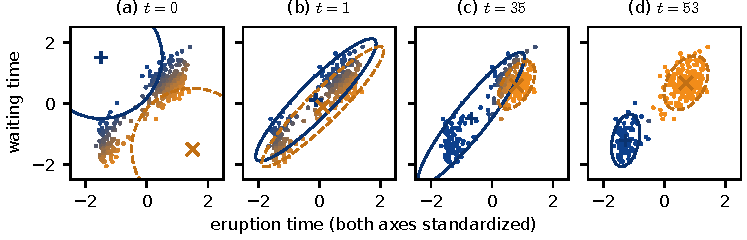
\includegraphics{em_iterations.pdf}
  \caption{EM on the standardized Old Faithful data, from equal weights,
    identity covariances and the means $(-1.5, 1.5)$ and $(1.5, -1.5)$,
    in the style of~\cite[Fig.~9.8]{bishop2006}: (a)~the start,
    (b)~after one iteration, (c)~after $35$, when $\ell$ has covered half
    of its climb, (d)~converged; $+$ and $\times$ mark the means. Each
    point is colored by its responsibilities, dark blue for the first
    component, orange for the second, and a mix when shared. The
    ellipses lie two standard deviations from the means: solid for the
    first component, dashed for the second.}
  \label{fig:iterations}
\end{figure}

\begin{table}[b]
  \centering\small
  \caption{The mixture fitted to the $272$ Old Faithful eruptions, in
    the original units: the weights $\pi_k$, the means of eruption time
    and waiting time in minutes, and the covariance entries in minutes
    squared, the variances $\sigma_{\mathrm{e}}^2$ of eruption time and
    $\sigma_{\mathrm{w}}^2$ of waiting time, and their covariance
    $\sigma_{\mathrm{ew}}$.}
  \label{tab:fit}
  \begin{tabular}{@{}ccccccc@{}}
    \toprule
    & & \multicolumn{2}{c}{mean} & \multicolumn{3}{c}{covariance} \\
    \cmidrule(lr){3-4}\cmidrule(lr){5-7}
    $k$ & $\pi_k$ & eruption & waiting
      & $\sigma_{\mathrm{e}}^2$ & $\sigma_{\mathrm{ew}}$
      & $\sigma_{\mathrm{w}}^2$ \\
    \midrule
    1 & 0.356 & 2.04 & 54.48 & 0.069 & 0.435 & 33.697 \\
    2 & 0.644 & 4.29 & 79.97 & 0.170 & 0.941 & 36.046 \\
    \bottomrule
  \end{tabular}
\end{table}

At the start, most points have a sizeable responsibility for both
components, so the first M-step gives both nearly the mean and the
covariance of all the points. The two ellipses almost coincide
(Figure~\ref{fig:iterations}(b)), and $\ell$ jumps from $-1331.48$ to
$-542.98$.

This is close to the identical components of Section~\ref{sec:theory},
and EM leaves them slowly (Figure~\ref{fig:loglik}(a)): $\ell$ covers
half of its climb from $-542.98$ to $-385.4607$ only at iteration $35$
(Figure~\ref{fig:iterations}(c)). On the way, $\ell$ still rose by at
least $0.035$ per iteration, far more than $\varepsilon$, so the
stopping test did not end the run on this plateau. Once the components
separate, the climb is fast, and EM stops after $53$ iterations, at
$\ell = -385.4607$ (Figure~\ref{fig:iterations}(d)). The smallest gain
of $\ell$ in one iteration is $2.2 \cdot 10^{-11}$, positive
(Figure~\ref{fig:loglik}(b)), so $\ell$ rose at every iteration,
consistent with Theorem~\ref{thm:ascent}, which requires only that it
never falls.

\begin{figure}[tbp]
  \centering
  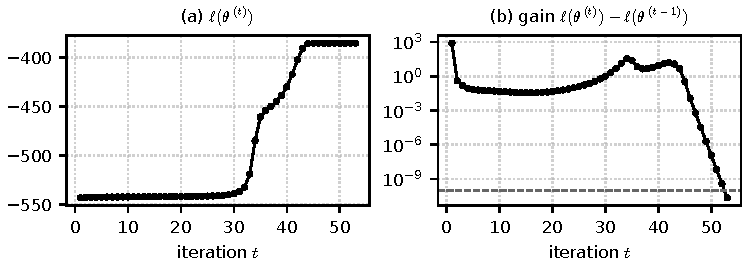
\includegraphics{em_loglik.pdf}
  \caption{The Old Faithful run of Figure~\ref{fig:iterations}:
    (a)~the log-likelihood $\ell(\theta^{(t)})$ for $t \geq 1$; (b)~the
    gain $\ell(\theta^{(t)}) - \ell(\theta^{(t-1)})$ of each iteration,
    on a log scale, with the tolerance $\varepsilon = 10^{-10}$ dashed.
    Panel~(a) leaves out the start, $\ell(\theta^{(0)}) = -1331.48$,
    for scale. Every gain is positive, small while the two components
    almost coincide and large once they separate; the last falls below
    $\varepsilon$ and ends the run.}
  \label{fig:loglik}
\end{figure}

The two components are the two groups of eruptions. The first, with
weight $0.356$, holds the short eruptions followed by short waits, the
second the long ones (Table~\ref{tab:fit}).

\subsection{Twenty random starts}\label{sec:starts}

Twenty random starts all reach the log-likelihood of the poor start; on
these data, the start changes the number of iterations, not the final
$\ell$. Each start has equal weights, identity covariances, and the
means at two data points chosen at random, with a fixed seed. Every run
stops at $\ell = -385.4607$, to four decimals, after $11$ to $37$
iterations, fewer than the $53$ of the poor start. None of them ends at
a stationary point with a different log-likelihood, although
Section~\ref{sec:theory} allows it. None of the $21$ final fits, the
poor start's and these twenty, collapses: the smallest covariance
eigenvalue, the smallest variance of a component in any direction, is
$0.047$, in standardized units.

%% ═══════════════════════════════════════════════════════════════════
\section{Conclusion}\label{sec:conclusion}

\begin{enumerate}[leftmargin=*, nosep]
\item EM fits a Gaussian mixture by alternating Bayes' rule for the
  hidden labels, the E-step~\eqref{eq:resp}, with weighted versions of
  the ordinary Gaussian fits, the M-step~\eqref{eq:mstep}.
\item One call of scikit-learn's \code{fit} reproduces the hand
  iteration to $6.2 \cdot 10^{-15}$, so the experiments run EM as
  derived.
\item On Old Faithful, $\ell$ rose at every iteration, consistent with
  Theorem~\ref{thm:ascent}; from a poor start, EM lingered near two
  identical components and converged after $53$ iterations.
\item All twenty random starts reached the same log-likelihood,
  $-385.4607$, in $11$ to $37$ iterations.
\end{enumerate}

The findings have limits: one data set, two components, one poor start
and twenty random ones; other data, more components or other starts can
end at other stationary points.

The same alternation of two steps underlies hidden Markov models and
linear-Gaussian state-space models, where the E-step is a
forward-backward recursion or a Kalman
smoother~\cite[Chapter~13]{bishop2006}. Todorović, Todorović-Zarkula
and Stanković~\cite{todorovic2012} treat Kalman-filter estimation of the
states and parameters of recurrent neural networks.

\section*{Code availability}

The notebook \nolinkurl{em_project.ipynb}, in the folder
\nolinkurl{project}, computes every number, table and figure in
Sections~\ref{sec:hand} and~\ref{sec:experiments}: NumPy and SciPy
compute the hand iteration, and scikit-learn runs EM. It runs on
Python~3.14.7 with NumPy~2.5.3, SciPy~1.18.1, scikit-learn~1.9.1 and
Matplotlib~3.11.2; these four, with ipykernel and nbconvert for the run
command, are pinned in \nolinkurl{project/requirements.txt}. With them
installed in a virtual environment \nolinkurl{project/.venv}, the
commands
\begin{center}\scriptsize
\begin{tabular}{@{}l@{}}
  \code{cd project}\\
  \code{.venv/bin/jupyter nbconvert -{}-to notebook -{}-execute
    -{}-inplace em\_project.ipynb}
\end{tabular}
\end{center}
run it; the run reported here took less than a minute. The public
repository \url{https://github.com/innicoder/em-algorithm-seminar} holds
this paper, its LaTeX source, the notebook with its outputs, and the
figures. The data file \nolinkurl{faithful.csv} in
\nolinkurl{project/data} is the data set \code{faithful} of R, from the
Rdatasets collection.

\printbibliography

\end{document}
